\documentclass[runningheads,a4paper]{elsarticle}
% vim: tw=0 wm=0

\setcounter{tocdepth}{3}
\usepackage{amssymb}
\usepackage{amsmath}
%\usepackage{amsthm}
\usepackage{bbm}
\usepackage{environ}
\usepackage{multirow}
\usepackage{longtable}
\usepackage{comment}
\usepackage{placeins}
\usepackage{mathtools}
%\usepackage{algorithmic}
\usepackage{enumitem}
\usepackage[utf8]{inputenc}
%\usepackage{enumite}
%\usepackage{cleveref}
%\usepackage{parskip}
\usepackage{algpseudocode}
\usepackage{algorithm}
\usepackage{array}
\usepackage[pdfencoding=auto,psdextra]{hyperref}
\usepackage{booktabs}
\usepackage{bookmark}% faster updated bookmarks
\usepackage{hypcap} % fix the links
\evensidemargin\oddsidemargin
\usepackage{graphicx}
\pagestyle{plain}
\usepackage{xcolor}
\newcommand\ToDo[1]{\textcolor{red}{#1}}
%\bibliographystyle{plainnat}
\usepackage{siunitx}
\usepackage{color}
\usepackage{epsfig}
\usepackage{caption}
\usepackage{subcaption}

\usepackage[draft,nomargin,inline]{fixme}
\fxsetface{inline}{\itshape}
\fxsetface{env}{\itshape}
%\fxuselayouts{margin}
%\fxuselayouts{inline}
\fxusetheme{color}

\usepackage{url}
\urldef{\mailsa}\path|{djukanovic, raidl}@ac.tuwien.ac.at,|
\urldef{\mailsb}\path|christian.blum@iiia.csic.es|
\newcommand{\keywords}[1]{\par\aDSvspace\baselineskip
	\noindent\keywordname\enspace\ignorespaces#1}

\usepackage{tikz}
\usetikzlibrary{positioning}
\definecolor{canaryyellow}{rgb}{1.0, 0.94, 0.0}
\definecolor{brightgreen}{rgb}{0.4, 1.0, 0.0}
\definecolor{jazzberryjam}{rgb}{0.65, 0.04, 0.37}

%defining of command

\newcommand\floor[1]{\lfloor#1\rfloor}
\newcommand\ceil[1]{\lceil#1\rceil}
\newcommand\str[1]{\texttt{#1}}
\newcommand\pL[1][]{\ensuremath{p^{\mathrm{L}#1}}}
\newcommand\pR[1][]{\ensuremath{p^{\mathrm{R}#1}}}
\newcommand\qL{\ensuremath{q^\mathrm{L}}}
\newcommand\qR{\ensuremath{q^\mathrm{R}}}
\newcommand\pLH{\ensuremath{\hat{p}^\mathrm{L}}}
\newcommand\pRH{\ensuremath{\hat{p}^\mathrm{R}}}
\newcommand{\Vext}{\ensuremath{V_\mathrm{{ext}}}}
\newcommand\UB{\ensuremath{\mathrm{UB}}}
\newcommand\Sigmand{\ensuremath{\Sigma^\mathrm{nd}}}
\renewcommand{\labelenumii}{\theenumii}
\renewcommand{\theenumii}{\theenumi.\arabic{enumii}.}
\setlength{\leftmarginii}{1.8ex}
\raggedbottom
\algnewcommand\algorithmicforeach{\textbf{for each}}
\algdef{S}[FOR]{ForEach}[1]{\algorithmicforeach\ #1\ \algorithmicdo}

% scaling factor for tables
\newcommand\tabscale{0.8}

\begin{document}
	
	%\setlength{\parindent}{0pt}  % disallow indentations
	%\numberwithin{table}{1}
	%\mainmatter  % start of an individual contribution
	
	% first the title is needed
	\title{Can greedy-like heuristics be useful for solving the Weighted Orthogonal Art Gallery Problem under regular grid discretization?}
	
	%
	\author[1]{Milan Predojevi\'c}
\author[1]{Marko Djukanovi\'c}
\author[1]{Milana Grbi\'c}
\author[1]{Dragan Mati\'c}
    \address[1]{Faculty of Natural Science and Mathematics, University of Banja Luka, Bosnia and Herzegovina}

	\begin{abstract}
		In this paper we deal with the Weighted Orthogonal Art Gallery Problem under the regular grid discretization. We propose a novel greedy approach which is based on balancing the trade off between the total sum of guards' costs and the total number of not yet covered points from the discretization. This new approach and an existing greedy algorithm are further  hybridized with the Integer Linear programming (ILP), originally formulated for the well known Minimum Set Cover problem. Experimental results show that the proposed greedy methods can achieve most of the optimal solution for a class of large area polygons, while for small area polygons, they achieve solutions of reasonable quality within lower runtime than the exact algorithms.
	\end{abstract}
	\maketitle
	
	
	\section{Introduction}\label{sec:introduction}
	
	Given a polygon $P$, the \emph{Art Gallery Problem} (AGP) asks for a set of points $G$ of minimal cardinality,  such that for each point $y \in P$ there is $x \in G$ such that $xy \subset P$. We say that the point $y$ is covered by the point $x$, or $y$ is visible from $x$. Set $G$ is called \emph{guard set} of $P$ and the points from $G$ as \emph{guards}. In the \emph{Orthogonal Art Gallery Problem} (OAGP) we suppose that edges of the polygon are only horizontal and vertical w.r.t. the axes, i.e.  the angles allowed between adjacent edges are  $90^{\circ}$ or $270^{\circ}$. The original AGP was initially stated by Victor  Klee in 1973.~\cite{o1987art}.  The problem is motivated from installing the cameras inside a building (or gallery) such that the whole area of the building is covered. Orthogonality constraint naturally comes out from the orthogonality of the walls in buildings. Kahn et al.~\cite{kahn1983traditional} formulated and proofed that 	$\lfloor \frac{n}{4} \rfloor$ guards are  sufficient to cover an orthogonal polygon with $n$ vertices.      In the course of this study, we are interested in the variant of the OAGP which allows only that guards are positioned at the vertices of polygon $P$. This restricted problem is known to be $\mathcal{NP}$--hard~\cite{schuchardt1995two,katz2008guarding}.  When it comes to the real situations (like installing the cameras in a building), it is justified to assume that the prices of cameras are not equal and may depends on several factors, like the quality of a camera   (respecting its range of spectrum of view)  or installation price at some specific parts of the building (like corners or tight places).  In the \emph{Weighted Orthogonal Art Gallery Problem} (WOAGP) the task is to place guards on some vertices of the orthogonal polygon which cover all points from $P$, such that the total sum of prices assigned to the chosen vertices is minimal. In this paper we consider WOAGP problem under the regular grid discretization of $P$, described in Subsection~\ref{sec:regulardiscretization}.
	
	It is well known that AGP can be reduced to \emph{the Minimum Set Cover Problem} (MSCP) by a discretization of the set of all points of the polygon $P$. The appropriate discretization should be performed in such a way that if each point from the discretized set $D(P)$ is covered, then the whole polygon $P$ is covered. After the discretization is made, for each vertex of polygon $P$, a set of visible points from $D(P)$ is determined. In that way, the problem of determining the minimum number of guards covering the entire polygon is reduced to determining the minimum number of subsets of points, such that each point from $D(P)$ is included in at least one of the chosen subsets, which is MSCP. Analogously, WOAGP can be reduced to the \emph{Minimum Weighted  Set Cover Problem} (MWSCP). 
	
	Concerning the exact and heuristic techniques to solve OAGP, Couto et al.~\cite{couto2007exact} presented an exact and efficient exact algorithm for the OAGP based on preprocessing and refinement phases of the the discretized instance. In ~\cite{ghosh2010approximation} an approximate solution of the minimum vertex guard problem, which can be computed in $O(n^4)$ time and the the solution is at most $O(\log n)$ times the optimal one. After that, on these constructed sets Johnson’s approximation algorithm ~\cite{johnson1974approximation} for the MSCP is applied. An anytime algorithm to compute successively better approximations of the optimum to Minimum Vertex Guard is proposed in~\cite{tomas2003approximation}.  A major idea of this approach is exploring dominance of visibility regions to first detect pieces that are
	more difficult to guard. The same problem is solved in~\cite{tomas2006visibility} by applying successive approximations from  ~\cite{tomas2003approximation}.
	Tozoni et al.~\cite{tozoni2013practical,tozoni2016algorithm}  presented an exact \emph{Integer Linear Programming}  (ILP)-based  algorithm, which iteratively generates upper and lower bounds through the resolution of discretized space of the AGP. Although many variants AGP are present in literature, WOAGP has not been so intensively studied, which motivated us to consider this problem.  A comprehensive analysis of various greedy-like heuristics for the MWSCP  was presented in \cite{vasko2016best}.
	More detailed overview of the extensive literature regarding MSCP and AGP is out of the scope of this paper and for further reading we suggest review papers ~\cite{caprara2000algorithms,ren2010new,ghosh2010approximation2}.

	
	\subsection{Main contributions}
	The main contributions of this paper are:
	\begin{itemize}
		\item We developed a novel greedy approach which is based on balancing the trade off between the total sum of guards' costs and the total number of not yet covered points from the discretization.
		\item The  greedy algorithm from \cite{chvatal1979greedy} and the novel greedy algorithm are hybridized with the ILP.
		\item We considered different types of weights for our benchmarks, based on an approximation of the costs in real situations.
		\item In a comprehensive computational experiment,  we tested, analysed and checked the efficiency of the developed algorithms. The methods are then compared to the exact approaches ILP and \emph{Constraint Programming} (CP) w.r.t. the quality of obtained heuristic solutions as well as runtimes.
	\end{itemize}

	
	\subsection{The Regular Grid Discretization of Polygon}\label{sec:regulardiscretization}
	Building of the regular grid discretization $D(P)$ of the polygon $P$ is shown in Algorithm \ref{alg:discret}.  At the beginning, the minimum bounding rectangle (usually called \textit{bounding box}) of $P$ is created. Then, the  regular grid, with resolution $\bigtriangleup_{x}\times\bigtriangleup_{y}$ and starting at the lower left corner of the bounding box of polygon $P$, is defined as follows:

	\begin{equation}
         \bigtriangleup_{x}=\min\{ |u_{x}-v_{x}|\mid u_{x}\neq v_{x}\} \mbox{ and }
         \bigtriangleup_{y}=\min\{ |u_{y}-v_{y}|\mid u_{y}\neq v_{y}\},
 	\end{equation}
where $ (u_{x},u_{y}),(v_{x},v_{y})$ are adjacent vertices of polygon $P$.
	
	\begin{algorithm}[!t]
		\caption{Discretization $D(P)$ of polygon $P$}\label{alg:discret}
		\begin{algorithmic}[1]
			\State \textbf{Input:} The set of vertices $V$ of polygon $P$
			\State \textbf{Output:} The discretization $D(P)$ of polygon $P$
			\State $BB \gets bounding\_box(P);$
			\State $\bigtriangleup_{x},\bigtriangleup_{y} \gets resolution(P);$
			\State $D(BB) \gets regular\_grid(BB,\bigtriangleup_{x},\bigtriangleup_{y});$
			\State $D(P) \gets D(BB) \cap P;$
			\State $D(P) \gets D(P) \cup V;$
		\end{algorithmic}
	\end{algorithm}
The algorithm further forms the whole regular grid of the bounding box (line 5 of the pseudocode) and finally, all points of the regular grid that belong to $P$ and all vertices of $P$ are added into the discrete set $D(P)$.
	
	It should be noticed that the optimal solution of WOAGP on $D(P)$ (i.e. an optimal covering of $D(P)$) is not necessarily  an optimal covering of $P$. In the simple example shown in Figure \ref{fig:example}, one can see that the guards placed on top left and top right vertices (shown in red color) cover all points from $D(P)$ (Figure \ref{fig:example} (a)), but not the whole polygon, since the gray triangle is not visible from any of these two points. The optimal solution value in this case is 1.2. Two red vertices in Figure \ref{fig:example} (b) optimally cover the whole polygon, but this covering is not optimal w.r.t. discrete set $D(P)$, since the total sum of weights is larger (1.6).
	
	\begin{figure}[t!]
    	\centering
    	\begin{subfigure}[t]{0.49\textwidth}
        	\centering
        	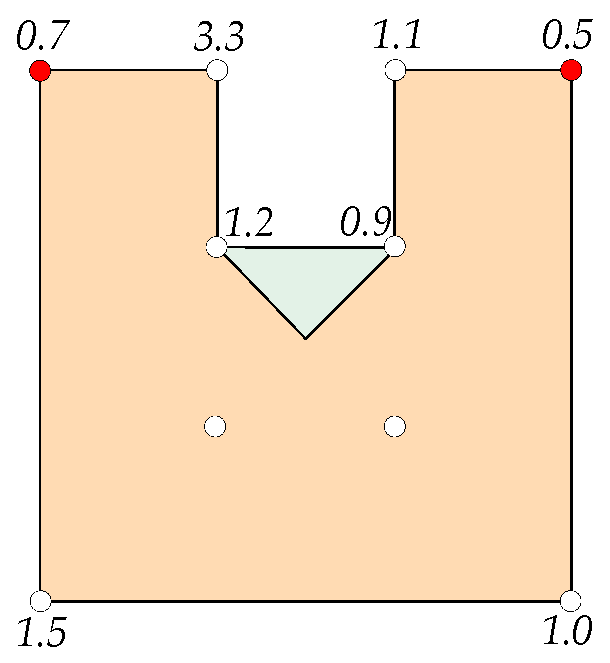
\includegraphics[height=1.7in]{slika1a.eps}
        	\caption{Optimal coverage of discretization $D(P)$. }
    	\end{subfigure}%
    	~
    	\begin{subfigure}[t]{0.49\textwidth}
        	\centering
        	\includegraphics[height=1.7in]{slika1b.eps}
        	\caption{Optimal coverage of polygon $P$.}
    	\end{subfigure}
    	\caption{Optimal coverage of discretization $D(P)$ does not imply a coverage of polygon $P$.}\label{fig:example}
	\end{figure}
	
	The chosen resolution  $\bigtriangleup_{x}\times\bigtriangleup_{y}$ is a compromise between the algorithm speed and accuracy. More precisely,  higher resolution increases the accuracy, but also the execution time and vice versa, lower resolution decreases the algorithm accuracy, but discretization is  generated faster.
	
	%Couto et al.~\cite{couto2007exact} koristili su pomenutu diskretizaciju za problem ortogonalne galerije. U njihovom radu broj pologona nad kojim je primjenjena ova diskretizacija je 10282. Za 59.4\% poligona je vazilo da iz pokrivenoosti diskretnog skupa D(P) slidi pokrivenost poligona P za optimalno pronadjen skup strazara koji pokrivaju D(P)\fxnote{Sta je sa ostalim poligonima koji nisu bili pokriveni?} Za ostale poligone je bilo potrebno dodati prosječno 0.003·n+1.1 dodatnih tačaka u diskretizaciju kako bi iz pokrivenosti diskretizacije slijedila pokrivenost poligona. Dakle nad testiranim uzorkom poligona, ili je citav poligon pokriven ili je mali broj regija nepokriveno optimalnim skupom stražara Z za D(P). U sekciji 4 će biti prikazane vrijednosti površina ovih nepokrivenih regija. \fxnote{Koliki je procenat pokrivenosti bio u tom slucaju?} \fxerror{Do ove info ne mogu da dodjem} \fxnote{Kako se ovo odnosi na druge diskretizacije, bilo je puno bolje ili?} \fxnote{Treba pregledati literaturu. Pitanje je koliko je ljudi pokusavalo ovom metodologijom dopunjavati diskretiyaciju kako bi dosli do optimalnog rjesenja - ja bih izbjegao o ovom pricati/pisati}.
	
	\section{Exact methods}
	In this section we present the exact ILP  initially developed for MWSCP from ~\cite{vazirani2013approximation} and \emph{Constraint Programming} (CP) models for solving WOAGP  under regular grid discretization, which are used  in the rest of the paper.
	\subsection{Integer linear programming model}
	Let us suppose we are given a polygon $P$ and the discretization $D(P)$ of $P$.  The task we consider is covering all points from $D(P)$ by some vertices $V=\{v_1,...,v_n\}$ of $P$ such that the sum of their weights is minimized.
	The problem is related to the known MWSCP  as follows.
	Family $\mathcal{F}$ of nonempty sets consists of the sets
	$S_i \in \mathcal{F}$ which include points $p \in D(P)$ that are visible from guard $v_i\in V$, i.e., $pv_i \subset P$.  For each set $S_i$, the cost $c(S_i) = w_i$ is assigned.  In this way, our starting task is equivalent of finding a  covering $\mathcal{C}\subseteq\{S_1,...,S_n\}$ of the set of points $D(P)$ of minimum weight, that is
	$$ \bigcup_{C \in \mathcal{C}} C = D(P),$$ such that

$$f(\mathcal{C}) = \sum_{S_i \in \mathcal{C}} c(S_i)$$

is minimized.

The ILP  model for the MWSCP ~\cite{vazirani2013approximation}   is  adapted to WOAGP  as follows:

	\begin{align}
	&\sum_{i=1}^n w_ix_i \longrightarrow \min  \label{eq:woagp-min}\\
	&\mbox{s.t.}\nonumber \\
	&\sum_{j=1}^n a_{ij}x_j \geq 1,\ (\forall p_i\in D(P)) \label{eq:const-3}\\
	& x_j \in \{0,1\},\ j\in\{1,2,\ldots,n\}\label{eq:const-4},
	\end{align}
	where
	$a_{ij} = \begin{cases}
	1, p_i \in S_j, \\
	0, \mbox{otherwise}.
	\end{cases}$
	 \\

	Set $Z = \{v_j \in V\mid x_j=1\}$ represents a solution of the problem w.r.t. discretization $D(P)$ of polygon $P$.
	Constraint~(\ref{eq:const-3}) enforces that any point $p_i \in D(P)$ will be visible from at least one guard from $Z$.
	
	In order to solve this model, we apply a general purpose solver \textsc{Cplex}~\cite{lima2010ibm}.
	\subsection{Constraint programming model} An equivalent CP model was implemented and tested by \textit{IBM ILOG CP Optimizer}~\cite{laborie2018ibm}. In this case,  Constraint~(\ref{eq:const-3}) is transformed into
	\begin{equation}
	\bigvee_{ j=1}^n (a_{ij} \wedge x_j) = 1, \forall p_i \in D(P),
	\end{equation}
	whereas the other constraints and the objective function are the same as in the above ILP model. Note that CP approach works in a branch-and-bound manner employing a constraint propagation and variable domain filtering~\cite{rossi2006handbook}.
	\section{Algorithmic Approaches for solving WOAGP}
	In this section we present the heuristic greedy approaches for solving WOAGP\fxnote{treba li ovdej w.r.t. regulagrid discrtization?} and their hybridization with the exact ILP method. 
	\subsection{Greedy approaches for solving WOAGP}
 Greedy algorithms produce a solution of reasonable quality within a short interval of time and are, in essence, easy to implement. Efficiency of such  heuristic is related to a greedy criterion utilized to expand current (non-complete, i.e., partial) solution to complete one. In order to extend current partial solution, among all candidates (solution components for expansion, that is not-yet-considered guards),  we choose one with the smallest greedy value and add it to the current solution. This procedure is repeating until the current solution becomes complete (i.e., all points from $D(P)$ are covered). 
 
 A general pseudocode of Greedy heuristics is given in Algorithm~\ref{alg:greedy}. 	The set Extend($s^{ps}$) includes those guards from set $V \setminus$ $s^{ps}$ that cover some points from $D(P)$ that are not yet covered by $s^{ps}$. Solution component of the problem is a guard. Extension of partial solution $s^{ps}$ by a vertex $v$ corresponds to adding $v$ into set $s^{ps}$.
	
	\begin{algorithm}[!t]
		\caption{Greedy Heuristic}\label{alg:greedy}
		\begin{algorithmic}[1]
			\State \textbf{Input:} an instance of a problem
			\State \textbf{Output:} A (feasible) non-expandable solution $s^{ps}$  (or reporting that no feasible solution exists)
			\State $s^{ps} \gets ()$ \hspace{0.3cm}// partial solution set to empty solution
			\While{$\text{Extend}(s^{ps}) \neq \emptyset$}
			\State Select solution component $e \in  \text{Extend}(s^{ps})$  \  w.r.t.\  some criterion $g$
			\State Extend $s^{ps}$ by $e$
			\EndWhile
		\end{algorithmic}
	\end{algorithm}
	\subsubsection{An existing greedy method}
	
	%  \subsection{Greedy Criterion based on Price-per-Unit}
	Concerning the greedy heuristic for the literature for solving MWSCP ~\cite{chvatal1979greedy, lovasz1975ratio}, one of the most efficient greedy heuristic was based on the following criterion:
	\begin{align}\label{eq:Lovasz}
	g_1(s^{ps}, v_i) = \frac{w_{i}}{ f(s^{ps} \cup \{v_i\})  - f(s^{ps})},
	\end{align}
	where
\begin{equation}\label{eq:sp}
    f(s^{ps}) = \left|\bigcup_{v_i \in s^{ps}} S_i \right|.
    \end{equation}
	This heuristic  also ensures an approximation with $O(\log(n))$ approximation factor.
	
	\subsubsection{A Novel Greedy Heuristic}
	In this subsection we present a novel greedy criterion. First, we introduce a term  ``incorrect point''. For a point from $D(P)$ we say that it is \textit{incorrect} if it is not covered by any guard from the current partial solution $s^{ps}$. Let us denote by $incorrect_{total}(s^{ps})$ the total number of incorrect points from discretization $D(P)$ w.r.t. $s^{ps}$. Note that
 \begin{equation}\label{eq:incorrect}
 incorrect_{total}(s^{ps}) = |D(P)|-f(s^{ps}),
 \end{equation}

 where $f(s^{ps})$ is defined in (\ref{eq:sp}) and $|D(P)|$ is the cardinality of discretization set. Let $w_{total}$ be the total sum of all weights among all vertices. The greedy function w.r.t. partial solution $s^{ps}$ and candidate guard $v$ is defined as follows.
	\begin{equation}\label{eq:greedyfun2}
    g_2(s^{ps}, v)  =    \frac{\sum_{i \in s^{ps} \cup \{v\}} w_i}{w_{total}}+ \frac{incorrect_{total}(s^{ps}\cup v)}{|D(P)|}.
	\end{equation}

	In the Equation  (\ref{eq:greedyfun2}) both terms are normalized on order to achieve better balance between the total sum of guards' costs and the total number of not yet covered points from the discretization. The algorithm does not  ultimately prefer any of criteria for choosing next vertex. Although it cannot be a rule, it is justified to suppose that the second term has a more influence on the choice of the next vertex in earlier phases of the algorithm execution. At the beginning, more points are uncovered and the algorithm  chooses such vertices which cover larger area of the polygon. At the end of algorithm, it could be expected that the first term plays more significant role, since the total number of uncovered points is small.
	
	
	Ties occurred in the search are broken by using  price-per-unit heuristic which is stated as follows.
	For each not yet considered vertex $v_i$, we denote the region of polygon $P$ that is visible from $v_i$ by $\emph{Surf}(v_i)$. As the next candidate to extend $s^{ps}$, we choose such a guard,  with the smallest ratio between the price and the visible surface area. More precisely, this  criterion is given as:
	\begin{align}
	g'(s^{ps}, v_i) = \frac{w_{i}}{|\emph{Surf}({v_i})|},
	\end{align}
    where $|\emph{Surf}({v_i})|$ represents the area of surface $\emph{Surf}({v_i})$.
	In our experimental studies, we found out that this heuristic does not perform well on its own, but it represents a reasonable tie-breaking mechanism which boosts quality of the aforementioned greedy heuristics.
	\subsubsection{Partial calculation of greedy functions}
	
	In order to enable fast calculation of greedy functions described in previous subsections, we noticed that it could be useful to allow fast updating of the number of uncovered vertices. Therefore, we introduced two useful structures: %and two auxiliary functions:
	\begin{itemize}
		%\item structure \texttt{map<Point,list<Point>> Visibility} -- for each point of $D(P)$, we provide the list of guards which are visible from that point;
		\item structure \texttt{numberOfGuards} -- which is a map structure, where each point from $D(P)$ is mapped to the number of guards in solution which cover that point;
		\item structure \texttt{CoveredPoints} -- as a set structure which keeps the points from $D(P)$ that are covered by the partial solution;
		%\item function \texttt{updateCoveredPointsAdd (vertex v)} -- does the update of  structures %\texttt{CoveredPoints} and \texttt{numberOfGuards} by considering only new points from $D(P)$ covered by vertex $v$, when $v$  is being added to partial solution; %pseudocode of the procedure is shown in Algorithm \ref{alg:updateCoveredPointsAdd}.
		%\item function \texttt{updateCoveredPointsRemove(vertex v)} -- does the update of structures \texttt{CoveredPoints} and \texttt{numberOfGuards} by removing all points which are covered only by $v$ , when $v$ is removed from partial solution; %pseudocode  is shown in Algorithm \ref{alg:updateCoveredPointsRemove}.
	\end{itemize}
  When adding vertex $v$ into partial solution, we update current \texttt{CoveredPoints} and \texttt{numberOfGuards} by considering only new points from $D(P)$ covered by $v$.
  When $v$ is removed from partial solution, we update current \texttt{CoveredPoints} and \texttt{numberOfGuards} by omitting all points which are covered only by $v$.  These two functions allow also a fast calculation of  functions (\ref{eq:sp}) and  (\ref{eq:incorrect}): a candidate vertex $v$ is temporary added to the partial solution, new status is checked and then being removed from the solution.


% Although the time complexity of both functions is $O(|D(P)|)$, % from Algorithms \ref{alg:updateCoveredPointsAdd} and \ref{alg:updateCoveredPointsRemove}
 % it is easy to notice that they only depends on the number of points covered by the current vertex, which is expected to be significantly lower than $|D(P)|$.


 \begin{comment}

	\begin{algorithm}[!t]
          	\caption{Function \texttt{updateCoveredPointsAdd}}\label{alg:updateCoveredPointsAdd}
          	\begin{algorithmic}[1]
          		\State \textbf{Input:} vertex $v$, $S[v]$:  list of points covered by $v$
          		\State \textbf{Output:} updated structures: coveredPoints and numberOfGuards
          		\For{$p$ in $S[v]$}
          		\State coveredPoints.insert($p$)
          		\State numberOfGuards.find($p$).second++
          		\EndFor
          	\end{algorithmic}
          \end{algorithm}

          %\begin{comment}

            \begin{algorithm}[!t]
          	\caption{Function \texttt{updateCoveredPointsRemove}}\label{alg:updateCoveredPointsRemove}
          	\begin{algorithmic}[1]
          		\State \textbf{Input:} vertex $v$, $S[v]$:  list of points covered by $v$
          		\State \textbf{Output:} updated structures coveredPoints and numberOfGuards
          		\For{$p \in S[v]$}
          		\State numberOfGuards.find($p$).second-- --
                \If {numberOfGuards.find($p$).second$=0$}
                    \State coveredPoints.remove($p$)
                    \EndIf
          		\EndFor
          	\end{algorithmic}
          \end{algorithm}
	  \end{comment}
 	
\subsection{A Hybrid of the \textsc{Greedy} and \textsc{Cplex}}
	The performance of \textsc{Cplex}  sooner or later degrades w.r.t. instance size due to the complexity of the problem. On the other hand, in the later stage, there is an increased chance for Greedy to worsen the obtained greedy solution due to an increased number of guards which are similar w.r.t. greedy value. So, it makes sense to combine  partial solutions generated with a Greedy procedure over a few iterations  and only then to make use the \textsc{Cplex} to do the completion of the partial solution. In details, our approach consists of the following steps:
	\begin{enumerate}
		\item Run a Greedy method up to $K$ iterations  to obtain a partial solution $s^{ps}$, where $K$ is a parameter of the algorithm.
		\item Take solution $s^{ps}$ and make it complete by solving a corresponding submodel via \textsc{Cplex}:
		\begin{itemize}
			\item \textsc{Cplex} solves corresponding sub-model which is formed by adding constraints $x_{i} = 1$, for all $v_i \in s^{ps}$ into the existing ILP  model~(\ref{eq:woagp-min})--(\ref{eq:const-4});
			\item a complete solution $\overline s$ is obtained;
		\end{itemize}
		\item Return $f(\overline s)$.
	\end{enumerate}
    This method is, therefore, called \textsc{Greedy}+\textsc{Cplex}.
	\begin{comment}
	
	\noindent \textbf{Improvements of the above method.} The above method can serve as a basic iteration
	of a more advanced techniques like ILP-LNS or CMSA. In this case, methods for destructing the solutions
	has to be proposed.  Underlying idea could be:
	\begin{itemize}
	\item remove $N$ guards with the largest costs out of $C'$
	\item remove $N$ guards which have a higher amount of points from $D(P)$ covered by other guards, represented by the function
	\begin{align}
	ratio(i) = \frac{\sum_{v \in V\setminus{ \{i\}}, j \in V(i)} 1_{j \mbox{ is veasible from } v} }{|V(i)|}.
	\end{align}
	\end{itemize}
	\end{comment}
	
	\section{Computational Results}

 We used two different kind of benchmark sets from~\cite{tomas2006visibility,bajuelos2004partitioning}: 
     \begin{itemize}
     	 \item \emph{MinArea} instances: MinArea includes polygons with a small areas and tiny interior. They present a lower boundary case for the cardinality of set $D(P)$ which means that, beside the polygon vertices,  $D(P)$ contains few additional points.
     	 \item \emph{FAT} instances:  includes polygons of large areas and wide interior. In this case,  a large number of points of regular grid is included into $D(P)$.
     \end{itemize}
     For each benchmark set -- \emph{MinArea} and \emph{FAT} instances -- one $n$-ogon for each $n \in\{8,10,...,200\}$ has been considered and the appropriate discretization is made, which makes 97 instances per each benchmark set. In overall, we have 194 instances. Discretization is performed by using \fxnote{nismo nigdje ubacili, a ovdje bi trebalo CGAL}.
     
	We included two kind of weights into each of 194  instances:
	\begin{itemize}
		\item \emph{topologically-based related weights} ($W0$): For each vertex $v_i$ of polygon $P$ we denote by $l_i$ and $l_{i+1}$ the lengths of two edges that come out of the vertex $v_i$. Then, we set 
\begin{equation}
w_i := \frac{l_i + l_{i+1}}{2}.
 \end{equation}
 This way of assigning weights is augmented by the fact that if the arithmetic length of both edges that comes out of vertex $i$ is longer, it is expected that a guard can see a larger pieces of polygon $P$. This implies that the spectrum of camera installed at $v_i$ has to be larger, which again implies that it should be of a higher quality, i.e,. a higher price.
		\item \emph{point-based related weights} ($W1$): For each vertex $v_j$, based on the number of points in $D(P)$ that are visible from $v_j$, we assign prices to each vertex on the following way:
		\begin{equation}
		w_i = n \cdot \frac{|S_i|}{|D(P)|},\ i=1,...,n.
		\end{equation}
    Similarly as in case of $W0$, cameras which cover larger range of points are considered be of a higher spectrum and quality, and thus are more expensive.
	\end{itemize}

     \subsection{Settings and the choice of the Parameters}
      All variants of our algorithms were implemented in C++ with g++~7.4 and the experiments were conducted in single-threaded mode on a machine with an Intel Xeon E5-2640 processor with 2.40 GHz and a memory limit of 8GB. The maximum computation time of each of our algorithms was set to $5\ min$.

      After conducting preliminary results, for
        \textsc{Greedy + \textsc{Cplex}} we decided to set up $K = \lceil 0.05 \cdot n \rceil$.

     The benchmark sets and the executable file of our software for this project are provided at \href{link}{link}. \fxnote{dodati link}
	\subsection{Results and Discussion}
        The following algorithms are included in our computation:
        \begin{itemize}
        	\item  exact approaches: CP and ILP approach. The later is, henceforth, called \textsc{Cplex};
            \item 4 heuristic approaches:
           \begin{itemize}
           	\item two pure greedy methods, guided by $g_1$ and $g_2$, labeled as \textsc{Greedy-1}, \textsc{Greedy-2}, respectively;
            %\item three \textsc{Greedy+Shaking} variants, henceforth labeled by \textsc{Greedy}-$i$+Shaking, $i=1,2,3$, where $i$ stands for heuristic $g_i$ involved in the method;
            \item two \textsc{Greedy+Cplex} variants, henceforth labeled by  \textsc{Greedy-1}+\textsc{Cplex} and
            \textsc{Greedy-2}+\textsc{Cplex}.
        \end{itemize}
    \end{itemize}


         Summarized numerical results for each of our 6 variants of our algorithm are displayed
         in Tables~\ref{small_wo} -- \ref{large_w1}. For each table, the average results are reported for each subset of instances grouped w.r.t. a specific kind of instances and a specific weight (97 instances per each group). Each of the tables list the tested algorithms in the first column. Starting with column two,  each of the lines provide detailed statistics for respective algorithm.  The statistics report: the average solution quality ($\overline{|s|}$), the average time ($\overline{t}[s]$) in seconds, the average number of guards which are included in each of the solutions ( $\overline{|g|}$), the number of solutions which match to the optimum solutions (\#optHit), average standard deviation of the obtained solutions w.r.t. optimal solutions ($\sigma(Opt)$), then the number of minimal solutions the algorithm obtained w.r.t. the four heuristics achieved by the respective algorithm (\#hitsMinH) and average standard deviation w.r.t. best (minimal) solutions achieved by the four heuristic algorithms   ($\sigma(MinH)$).  An asterisk in front of a number means that the exact approach  could prove optimality in all cases. Best values among heuristic approaches in each column are bolded.


     \begin{table}[]
     	\centering
     	 \scalebox{0.83}{
     	\begin{tabular}{l|lllllll}    \hline
     		Alg.           & $\overline{|s|}$ & $\overline{t}[s]$ &   $\overline{|g|}$ &optHit & $\sigma(Opt)$ & \#hitsMinH & $\sigma(MinH)$ \\ \hline
     		\textsc{Cplex}            & *15.93  & 0.152    & 18.93     & 97/97     & 0.00    & N/A        & N/A      \\
     		\textsc{Cp}               & 16.04  & 98.215   & 18.96     & 67/97     & 0.02    & N/A        & N/A      \\ \hline
     		\textsc{Greedy-1}             & 22.63  & \textbf{0.002}    & 26.28     & 0/97      & 0.79    & 3/97       & 7.61     \\
     		\textsc{Greedy-2}          & 19.97  & \textbf{0.002}    & 20.14     & 0/97      & 0.44    & 0/97       & 0.20     \\
     		   \textsc{Greedy-1+Cplex}  & 18.49  & 0.073    & 21.19     & \textbf{2/97}      & 0.30    & \textbf{57/97}      & \textbf{0.06}     \\
     		   \textsc{Greedy-2+Cplex} & \textbf{18.39}  & 0.004    & \textbf{19.59}     & 0/97      & \textbf{0.26}    & 53/97      & 0.04  \\ \hline
     	\end{tabular}}
        \caption{The results on the benchmark set $MinArea$ for the type of weight $W0$.}\label{small_wo}
     \end{table}

      \begin{table}[]
      	\centering
      	\scalebox{0.83}{
      	\begin{tabular}{l|lllllll} \hline
      		Alg.           & $\overline{|s|}$ & $\overline{t}[s]$ &  $ \overline{|g|}$ &optHit & $\sigma(Opt)$ & \#hitsMinH & $\sigma(MinH)$ \\ \hline
      		\textsc{Cplex}            & *36.03  & 0.003   & 18.93     & 97/97     & 0.00    & N/A        & N/A      \\
      		\textsc{Cp}               & *36.03  & 18.953   & 18.93     & 97/97     & 0.00    & N/A        & N/A      \\ \hline
      		\textsc{Greedy-1}             & 39.28  & \textbf{0.001}    & 20.15     & 2/97      & 0.35    & 4/97       & 0.24     \\
      		\textsc{Greedy-2}          & 40.92  & \textbf{0.001}    & 20.96     & 0/97      & 0.51    & 0/97       & 0.40     \\
      		   \textsc{Greedy-1+Cplex}  & 37.78  & 0.006    & 19.41     & \textbf{4/97}      & 0.21    & 19/97      & \textbf{0.08}     \\
      		   \textsc{Greedy-2+Cplex} & \textbf{37.31}  & 0.003    & \textbf{19.58}     & 2/97      & \textbf{0.15}    & \textbf{81/97}     & {0.19}   \\ \hline
      	\end{tabular}}
         \caption{The results on the bemchmark set $MinArea$ for the  type of weight $W1$.}\label{small_w1}
      \end{table}

     \begin{table}[]
      \centering
       \scalebox{0.85}{
     	\begin{tabular}{l|lllllll} \hline
     		Alg.           & $\overline{|s|}$ & $\overline{t}[s]$ &   $\overline{|g|}$ &optHit & $\sigma(Opt)$ & \#hitsMinH & $\sigma(MinH)$ \\ \hline
     		\textsc{Cplex}            & *2.62   & 0.02    & 7.32      & 97/97     & 0.00    & N/A        & N/A      \\
     		\textsc{Cp}               & *2.62   & 8.17    & 7.32      & 97/97     & 0.00    & N/A        & N/A      \\ \hline
     		\textsc{Greedy-1}             & 3.39   & 0.35    & 7.81      & 0/97      & 0.09    & 23/97      & 0.05     \\
     		\textsc{Greedy-2}          & 3.52   & \textbf{0.32}    & 6.61      & 2/97      & 0.10    & \textbf{28/97}      & 0.08     \\
     		   \textsc{Greedy-1+Cplex}  & 3.34   & 0.35    & 8.91      & 4/97      & \textbf{0.08}    & 25/97      & \textbf{0.04}     \\
     		   \textsc{Greedy-2+Cplex} & \textbf{3.32}   & 0.33    & \textbf{6.81}      & \textbf{6/97}      & \textbf{0.08}    & 25/97      & \textbf{0.04}  \\ \hline
     	\end{tabular}}
          \caption{The results on the benchmark set $FAT$ for the type of weight $W0$.} \label{large_w0}
     \end{table}

    \begin{table}[]
    	\centering
    	\scalebox{0.85}{
 	  \begin{tabular}{l|lllllll} \hline
 		Alg.           & $\overline{|s|}$ & $\overline{t}[s]$ &   $\overline{|g|}$ & optHit & $\sigma(Opt)$ & \#hitsMinH & $\sigma(MinH)$ \\ \hline
 		\textsc{Cplex}            & *6.72   & 0.02    & 6.44      & 97/97     & 0.00    & N/A        & N/A      \\
 		\textsc{Cp}               & *6.72   & 0.36    & 6.44      & 97/97     & 0.00    & N/A        & N/A      \\ \hline
 		\textsc{Greedy-1}             & 6.77   & \textbf{0.31}    & 6.49      & 92/97     & 0.02    & 92/97      & 0.04     \\
 		\textsc{Greedy-2}          & 6.77   & \textbf{0.31}    & 6.49      & 92/97     & 0.02    & 92/97      & 0.04     \\
 		\textsc{Greedy-1+Cplex}  & \textbf{6.73}   & 0.32    & \textbf{6.45}      & \textbf{96/97}     & \textbf{0.01}    & \textbf{96/97}      & \textbf{0.03}     \\
 		\textsc{Greedy-2+Cplex} & 7.42   & \textbf{0.31}    & 6.46      & 90/97     & 0.33    & 92/97      & 0.33    \\ \hline
 	\end{tabular}}
    \caption{The results on the benchmark set $FAT$ for the type of weight $W1$.}\label{large_w1}
   \end{table}

        From the numerical results, we observe the following conclusions concerning exact solving:
        \begin{itemize}
        	\item  \textsc{Cplex} could solve all solution to prove optimality within a fraction of a second;
        	\item   \textsc{Cp} was able to solve all those instances with weight $W1$ but with significantly more time than the time required from \textsc{Cplex};
        	\item For the subset of instances $MinArea$ which includes weight $W0$, the performance of Cp degrades significantly, which can be seen  by the respective average runtime and the number of proven optimal solutions found (67/97).
        \end{itemize}
     From the numerical results, we observe the following conclusions concerning heuristic solving:
     \begin{itemize}
     	\item  In case of the instances that include small--area polygons ($MinArea$) and weight $W0$ (Table~(\ref{small_wo})): A novel \textsc{Greedy-2} was able to significantly outperform the \textsc{Greedy-1} from literature. In this case, the best performing heuristic algorithms is hybrid \textsc{Greedy-2+Cplex} which needs the two order of magnitude lower average runtime to finish than the pure greedy methods. The average runtimes of all four heuristic methods are an order of magnitude lower than the average runtime of \textsc{Cplex}. Pure greedy methods deliver solutions of reasonable quality within 20\% of the quality of optimal solutions but needs the time which is 7-8 times lower then the average runtime of \textsc{Cplex}. Although all heuristic methods could not achieve optimal solutions (with the exception of two cases for \textsc{Greedy-1+Cplex} heuristics), the average standard deviation w.r.t. optimal solution is rather small. From last two columns, it is evident that both hybrid variants are more successful, hitting more than a half best solution each, with very small average standard deviation w.r.t. optimal solutions.
     	\item  In case of the instances that include small-area polygons and weight $W1$ (Table~\ref{small_w1}): the best heuristic approach is \textsc{Greedy-2+Cplex} which is able to deliver solutions which are within 3\% of the optimum ones. Note that in 81 cases (out of 91) \textsc{Greedy-2+Cplex} is able to deliver equally good or better results that the other heuristic approaches. As it was the case  of the weight $W0$, heuristic methods could not achieve many optimal solutions, but the obtained  average standard deviation w.r.t. optimal solutions is rather small.
     	The results of pure greedy method \textsc{Greedy-1} outperform the results of \textsc{Greedy-2}. These two methods are effective since they deliver solutions which are within 10\% of the \textsc{Cplex} results but need 3 times less runtime. The results of \textsc{Greedy-1} match just in two cases to the optimum.
     	
     	\item In case of the instances that include large-area polygons ($FAT$) and weight $W0$ (Table~ \ref{large_w0}): the exact \textsc{Cplex} approach is a clear winner concerning average solutions' quality as well as the average runtimes;  the best heuristic algorithm w.r.t. solution quality is \textsc{Greedy-2 +Cplex}. It also matches in more cases (on 6 instances) to the optimum result then the other heuristic approaches. The obtained average results are within 22\% of the average of  optimal solutions.  The pure \textsc{Greedy-1} slightly outperforms the pure greedy \textsc{Greedy-2}. It is interesting that \textsc{Greedy-1} assigns in average a  higher number of guards in solutions when compared to the average number of guards of \textsc{Greedy-2}. The runtimes of our heuristic approaches are an order of magnitude lower than the time of \textsc{Cplex} approach. Reason for that can be seen in the used regular discretization of the polygon. For the polygons with a larger area, more points are involved in the discrete set $D(P)$ and, therefore, iterations of greedy methods take a longer time than in case when $D(P)$ is smaller (which was the case of \emph{MinArea} polygons).
     	\item  In case of the instances that include large-area polygons ($FAT$) and weight $W1$ (Table~(\ref{large_w1}): the best heuristic algorithms w.r.t. solution quality is \textsc{Greedy-1+Cplex} which is able to match in 96 instances the quality of optimal solutions. Slightly worse results are delivered by \textsc{Greedy-1} and \textsc{Greedy-2}. The obtained (heuristic) solutions of these two approaches are within 1\% of optimal solutions and they are
     	able to reach the quality of the optimal solution for 92 instances. Unfortunately, the runtimes in comparison to the runtimes of \textsc{Cplex} are significantly higher for all of our heuristic approaches. However, the average runtime for \textsc{Cp} is a bit higher that the avg. runtimes of the heuristic approaches. Again, average standard deviation for each heuristic method is rather small w.r.t. optimal solutions, indicating good quality of the proposed algorithms.
     	\item  Concerning the percentage of covering of polygons for the best solutions (found by \textsc{Cplex}) we
     	noticed that  \textsc{FAT} instances are covered in almost all cases (see Fig.\ref{fig:covw0} and \ref{fig:covw1} and the blue curve). Concerning the \textit{MinArea} instances, it gets harder to cover all polygon and in allmost all cases the whole area of polygon $P$ cannot be covered. For these instances, we see that the solutions cover more regions of small--area polygons when weight $W1$ is considered then when considering $W0$ ($\approx 93 \%$ vs. $\approx 85\%$). It can be argued by the fact that in weight $W0$ there exists many ties for weights of guards, and, therefore, more solutions with the minimum weight exist.
     	Notice that this is not so often the case of the weight $W1$.
     	
     \end{itemize}


    \begin{figure}[!ht]
    	\centering\scalebox{0.9}{
    	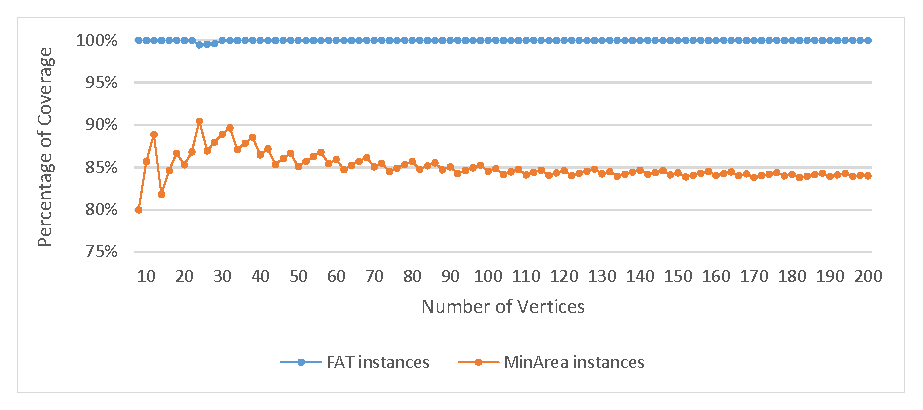
\includegraphics[width=\textwidth]{grafikon1.eps}}
    	\caption{Polygon coverage for the type of weight W0.}
    	\label{fig:covw0}
    \end{figure}

    \begin{figure}[!ht]
    	\centering
    	\centering\scalebox{0.9}{
    	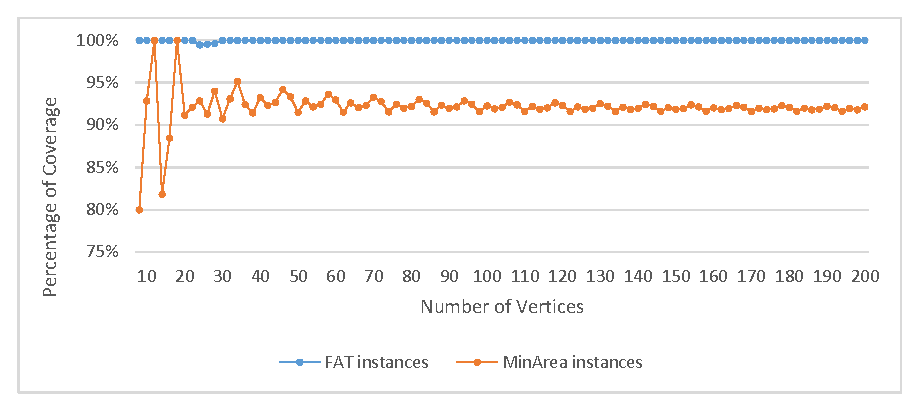
\includegraphics[width=\textwidth]{grafikon2.eps}}
    	\caption{Polygon coverage for the type of weight W1.}
    	\label{fig:covw1}
    \end{figure}

    \begin{figure}[!ht]
    	\centering
    	 \scalebox{0.9}{
    	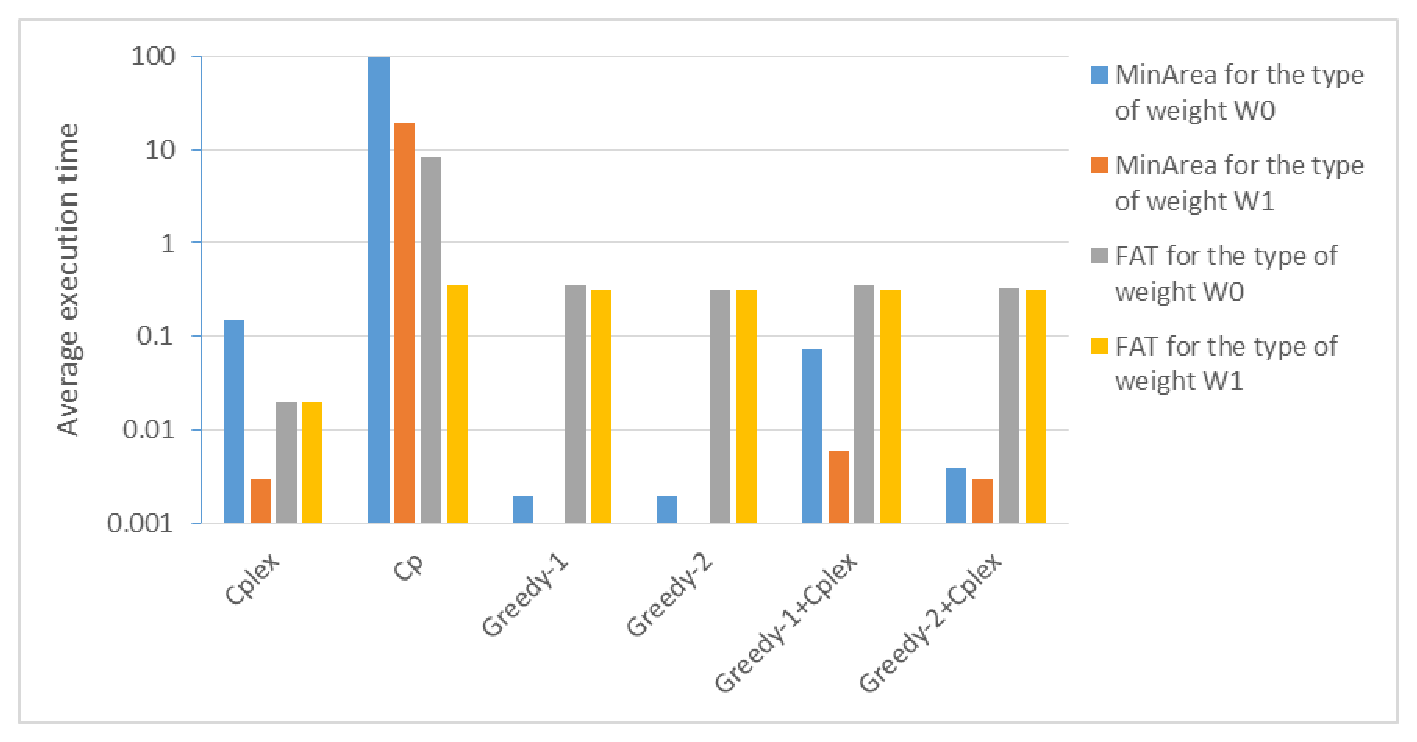
\includegraphics[width=\textwidth]{grafikon3.eps}}
    	\caption{Avg. execution time of the compared algorithms.}
    	\label{fig:timealg}
    \end{figure}


	\section{Conclusions and Future Work}
	  In this work we have considered the Weighted Orthogonal Art Gallery Problem under regular grid discretization.
	  We have developed a novel greedy criterion which provide a trade-off between the number of guards and the cost of  guards. Moreover, a hybrid of a greedy method and \textsc{Cplex} was proposed to make a maximal completion of the greedy solution obtained by the greedy method supplemented by solving respective subproblem via \textsc{Cplex}. The performances of the heuristic approaches are compared to the exact ILP and CP approaches. From the computational experiments, the heuristic approaches were highly efficient in terms of obtaining solutions of reasonable quality in an order of magnitude lower runtime than the exact approaches for the small-area polygons. For the large--area polygons, heuristic approaches were able to reach the quality of optimal solutions in almost all cases but in cost of larger times than the times of the ILP approach.
	
	  For the future work, we tend to improve the results of our greedy method as well as runtimes on the $FAT$ benchmark sets by considering different discretizations of polygons, for example, the Delaunay triangulation~\cite{lee1980two}.
	
	
	
	\section*{Acknowledgements}
This research is partially supported by Ministry for Scientific and Technological
Development, Higher Education and Information Society, Government
of Republic of Srpska, B\&H under the Project \fxnote{ime projekta}.

	
	\section*{References}
	\bibliographystyle{abbrv}
	\bibliography{bib}
	
	
\end{document}
